% !TEX program = xelatex
\documentclass[a4paper,UTF8]{article}
\usepackage[version=4]{mhchem}
\usepackage[UTF8]{ctex}
\usepackage{fontspec}
\usepackage{geometry}
\usepackage{tcolorbox}
\usepackage{graphicx}
\setmainfont{SimSun}
\setlength{\parindent}{0em}
\setlength{\fboxsep}{1em}
\geometry{textwidth=15cm}
\geometry{hcentering}
\begin{document}
\begin{center}
{\huge 我的化学笔记}

author:zzy
\end{center}

\section{氢和稀有气体}
稀有元素:自然界中含量少和分布稀少,被人们发现较晚,难以从矿物中提取或是在工业上制备和应用较晚的元素
\subsection{稀有元素分类}
稀有元素:

(1)轻稀有元素:Li,Rb,Cs,Be

(2)分散性稀有元素:Ga,In,Tl,Se,Te

(3)高熔点稀有元素:Ti,Zr,Hf,V,Nb,Ta,Mo,W

(4)稀土元素:Sc,Y,La及镧系元素

\subsection{化合态和游离态}
游离态:

(1)气态非金属单质

(2)固态非金属单质

(3)金属单质

注:

过冷状态:液态物质在温度降低到凝固点而仍不发生凝固或结晶等相变的现象。(Cs,Ga)


\subsection{单质的制取方法}
1.物理分离法

淘洗黄金,分离氧气氮气

2.热分解法

热稳定性差的某些金属化合物直接加热

$$ \ce{2Ag2O ->[\Delta] 4Ag(s) + O2}$$
$$ \ce{HgS(s) + O2 ->[\Delta]  Hg(l) + SO2(g)}$$

热分解法还用于制备某些高纯单质

$$ \ce{Zr(\text{粗}) + 2I2 ->[600^\circ C] ZrI4 ->[1800^\circ C] Zr(\text{纯}) + 2I2} $$
3.还原法

使用还原剂制取单质的方法叫做还原法。

$$ \ce{MgO(s) + C ->[\Delta] Mg + CO\ce{^}}$$
$$ \ce{Fe2O3 + 2Al ->[\Delta] 2Fe + Al2O3} $$

4.电解法

活泼金属和非金属单质的制备可采用电解法。

$$ \ce{2Al2O3(\text{熔体}) ->[\text{电解}][Na3AlF4,960^\circ C] 3S + 2H2O} $$ 

5.氧化法

用氧化剂制取单质的方法。如制取S:

$$ \ce{3FeS2 + 6C + 8O2 ->[\Delta] Fe3O4 + 6CO2\ce{^} + 6S\ce{^}} $$

也可从\ce{H2S}制取S:

$$ \ce{2H2S + 3O2 -> 2SO2 + 2H2O} $$
$$ \ce{ 2H2S + SO2 ->[CaT][300^\circ C] 3S + 2H2O} $$

\subsection{氢}
\subsubsection{氢原子的成键效应}

1.失去价电子

\ce{H+}半径小,具有很强电场,极化作用很强。

2.结合一个电子

这是\ce{H}与活泼金属形成离子型氢化物如\ce{NaH}、\ce{CaH2}的成键特征

3.形成共价化合物

与其他非金属形成共价型氢化物(\ce{HCl}、\ce{H2S}、\ce{NH3})。

\subsubsection{氢的性质和用途}

性质:

1.溶解度:氢在水中溶解度很小,在金属中溶解度却很大。

2.活泼性:在常温下不活泼。原因是氢原子半径小,无内层电子,所以共用电子对直接受核作用,形成的$\sigma$键很牢固,\ce{H2}的解离能很大。

3.与金属:加热时,与碱金属、碱土金属化合形成离子型氢化物(性质见碱金属/碱土金属部分);\\在过渡型氢化物中,氢以三种形式存在:\\·原子状态存在于金属晶格中\\·氢的价电子进入氢化物导带,以\ce{H+}形式存在\\·氢从氢化物导带中得一个电子,以\ce{H-}形式存在\\高温下,\ce{H2}作为还原剂与氧化物或氯化物反应,还原某些金属和非金属。


用途:

氢的扩散性好,导热性强;熔沸点均低,难液化,可作超低温制冷剂;热值高可作高能燃料。

与碱金属、碱土金属化合形成离子型氢化物(性质见碱金属/碱土金属部分)

化工上,氢气和用于生产甲醇。
$$ \ce{CO(g) + 2H2(g) ->[\text{催化加压}][\text{加热}] CH3OH} $$

食品工业上,则可用于有机物催化加氢。


$$ \ce{WO3 + 3H2 ->[\text{高温}] W + 3H2O} $$
$$ \ce{SiHCl3 + H2 ->[\text{高温}] Si + 3HCl} $$

4.与非金属:绝大多数p区元素与\ce{H2}反应生成共价型氢化物,它们在固态多数属于分子晶体,故又称分子型氢化物;它们大多是无色的,熔沸点较低;它们的物理性质相似,但化学性质显著不同。

5.检验:氢气能让粉红色\ce{PdCl2}水溶液迅速变黑(析出金属钯粉)

$$ \ce{PdCl2(aq) + H2(g) ->[\text{高温}] Pd(s)\ce{v} + 2HCl(aq)} $$

6.温度影响:高温下,氢分子分解为原子氢,具有极强还原性。

\subsubsection{氢气的制备}

实验室里,用\ce{Zn}与盐酸、稀硫酸作用制取氢气;

军事上使用\ce{CaH2}与水反应制取氢气。

工业上,主要有:

1.矿物燃料转化法:

制备水煤气:

$$ \ce{CH4(g) + H2O(g) ->[CaT][700-800^\circ C] CO(g) + 3H2} $$
$$ \ce{C(s) + H2O(g) ->[1000^\circ C] CO(g) + H2(g)} $$

将水煤气与水蒸气反应

$$ \ce{CO(g) + H2O(g) ->[400-600^\circ C][\ce{Fe},\ce{Cr}\text{催化剂}] CO2(g) + H2(g)} $$

本质上,每一步都是在让\ce{C}夺走水中的\ce{H}

该法制氢伴随大量\ce{CO2}产生。

2.电解法

电解\ce{NaOH}溶液,则在阴极产生氢气,阳极产生氧气。

\subsection{稀有气体}

稀有气体:0族元素所对应的气体单质。

\subsubsection{稀有气体的性质和用途}

稀有气体原子间存在微弱的色散力,作用力随着原子序数增大而增大(因为分子变形性增大)。所以,稀有气体的物理性质(熔沸点、临界温度、溶解度)也随着原子序数增大而增大。

1.氦(\ce{He})

用来代替氧气瓶中\ce{N2},防止潜水员“潜水病”。

2.氖(\ce{Ne})和氩(\ce{Ar})

霓虹灯、保护气、冷冻剂。

3.氪(\ce{Kr})和氙(\ce{Xe})

特种光源、麻醉剂。

4.氡(\ce{Rn})

有放射性,可用于放疗。

\subsubsection{稀有气体化合物}
第一个稀有气体化合物:

$$ \ce{Xe(g) + PtF6(g) -> Xe+[PtF6]-(s)} $$

现在,有稀有气体卤化物、氧化物、含氧酸盐等,大多都与氟化物的反应有关。

稀有气体氟化物:

$$ \ce{Xe(g) + F2(g) -> XeF_{x}(g)} $$

根据\ce{F}的用量和时间长短,可分别制得$x=2,4,6$的化合物;反应中若进入湿气,则生成爆炸的\ce{XeO3}。

\ce{XeF2}与水反应生成\ce{Xe}和\ce{HF}、\ce{O2};\ce{XeF4}、\ce{XeF6}则与水反应生成固态的\ce{XeO3}

\ce{Xe}的氟化物是优良的氟化剂,如:

$$ \ce{Pt + XeF4 -> PtF4 + Xe} $$

\ce{Xe}的三种氟化物均为强氧化剂,如:

$$ \ce{XeF2 + H2O2 -> Xe + 2HF + O2\ce{^}} $$

$$ \ce{6HCl + XeF6 -> 3Cl2\ce{^} + 6HF + Xe} $$

$$ \ce{6HCl + XeF6 -> 3Cl2\ce{^} + 6HF + Xe} $$

需要注意的是\ce{Xe}的氟化物的分子结构。\ce{XeF4}中有中心原子的8个电子,每个\ce{F}原子提供一个价电子,价层有$\frac{8+(4\times1)}{2}=6$对电子,为八面体结构。两对孤电子占据对角,四个成键电子对占据四个顶点,为正方形,\ce{Xe}位于正方形中心。



\section{碱金属和碱土金属元素}

\subsection{碱金属和碱土金属通性}

$IA$和$IIA$族元素均只有1到2个s电子,同一周期中,半径大、电荷少。所以,它们的金属晶体中金属键不牢固,单质熔沸点低,硬度小。由于碱土金属比碱金属原子半径小、原子电荷多,因此碱土金属的熔沸点都比碱金属高,密度、硬度都比碱金属大。

总的来说,从上到下熔沸点降低、密度增加、硬度减小、电负性降低、$E^{\theta}(\ce{M2+}/\ce{M})$绝对值增加,还原性增加。

然而,\ce{Li/Li+}的标准电极电势反常,这是因为其原子半径小,很容易与\ce{H2O}结合放出能量,水合焓代数值最小导致的。研究反应的焓变,可以得到如下过程。

\begin{figure}[htpb]
	\centering
	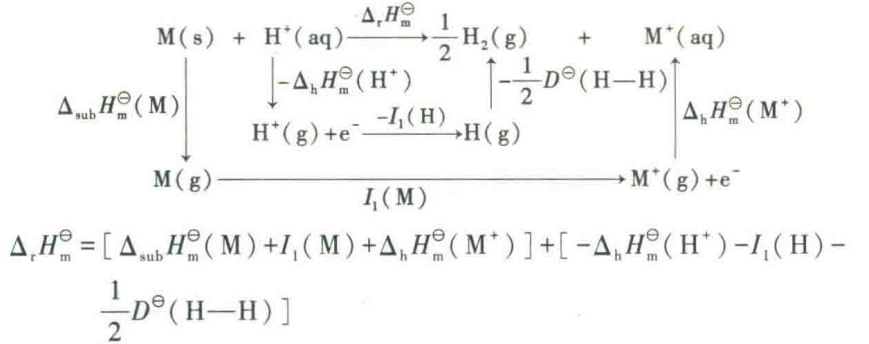
\includegraphics[width=0.5\textwidth]{figure//Li的电极电势反常的原因.png}
	\caption{Li的水合焓对焓变的影响}
	\label{fig:}
\end{figure}

\begin{tcolorbox}

%\begin{figure}[htpb]
%	\centering
%	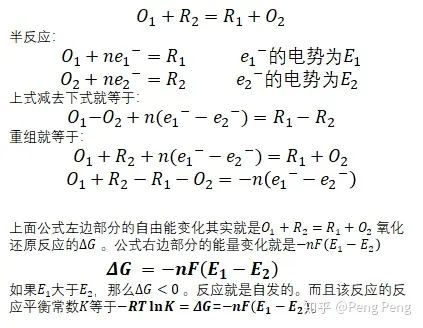
\includegraphics[width=0.5\textwidth]{figure//电势与Gibbs自由能.png}
%	\caption{电势与Gibbs自由能的关系}
%	\label{fig:}
%\end{figure}

如何描述Gibbs自由能与电势的关系:

例如,对于反应

$$ \ce{O1 + R2 = R1 + O2} $$

半反应:

$$ \ce{O1 + ne1^- = R1 \quad potential\ of\ e1^- = E_1} $$

$$ \ce{O2 + ne2^- = R2 \quad potential\ of\ e2^- = E_2} $$

上式减下式就等于(注意,此处从左到右均为还原反应):

$$ \ce{O1 - O2 + n(e1^- - e2^-) = R1 - R2} $$

重组就等于:

$$ \ce{O1 + R2 - R1 - O2 = -n(e1^- - e2^-)} $$

上面公式左边部分的变化就是 $ \ce{O1 + R2 = R1 + O2} $ 氧化还原反应的 $ \Delta G $。公式右边部分的能量变化就是$ -nF(E_1 - E_2) $

$$ \ce{\Delta G = -nF(E1 - E2)} $$

若$ E1 > E2 $,那么$ \Delta G < 0 $。反应就是自发的。而且反应平衡常数有 $ -RTlnK = \Delta G = -nF(E1 - E2) $值得注意的是,此处$E_1$为原反应的还原部分,而$E_2$为氧化部分。\\

电动势的本质,就是两个电极之间各物质的电化学势能(electromical potential)总和达到平衡,测量出的电子在两端电极的电势能之差。

关于电化学势能,它与物质的活度、带电荷数有关。

\end{tcolorbox}

碱金属和碱土金属均可溶于液氨,生成溶剂合电子和阳离子,形成具有导电性的深蓝色溶液。

$$ 碱金属:\ce{M(s) + (x+y)NH3 <=> M+(NH3)x + e-(NH3)y}(蓝色) $$

$$ 碱土金属:\ce{M(s) + (x+2y)NH3 <=> M^2+(NH3)x + 2e-(NH3)y}(蓝色) $$

碱金属、碱土金属的氨溶液具有导电性,可发生于金属本身类似的化学反应,例如钾的液氨溶液可还原\ce{Ni(II)},制得\ce{Ni(I)}配合物:

$$ \ce{2K2[Ni(CN)4] + 2K+(NH3) + 2e-(NH3) ->[-30^\circ C below][NH3(l)] K4[Ni2(CN)6](NH3)4 + 2KCN} $$

碱金属和碱土金属氨溶液不稳定,可以被催化为氨基化物(阳离子与氨基连接):

$$ \ce{Na+(NH3) + e-(NH3) ->[FexOy] NaNH2(NH3) + \frac{1}{2}H2(g)} $$

碱金属可以溶于醚和烷基胺中。

碱金属和碱土金属可以与\ce{H2,H2O,X2,N2,S,O2}反应,其中与\ce{N2}反应的有\ce{Li,Mg,Ca,Sr,Ba};与\ce{H2O}反应的有碱金属,\ce{Ca,Sr,Ba,Mg}。

\subsection{氢化物}

碱金属和碱土金属加热时与氢直接化合,形成离子型氢化物,其中氢为-1价。

所有纯的离子型氢化物都是白色晶体,不纯的为浅灰色至黑色。性质类似盐,又称为类盐型氢化物,密度比相应金属密度大得多。

类盐型氢化物:碱金属和碱土金属与氢化合形成的离子型氢化物。

离子型氢化物受热分解为氢气和游离金属。

$$ \ce{2MH ->[\Delta] 2M + H2\ce{^}} $$

离子型氢化物与水反应生成氢气,原因是\ce{H-}与水中\ce{H+}结合为\ce{H2}。

$$ \ce{LiH + H2O -> LiOH + H2\ce{^}} $$

离子型氢化物都是极强的还原剂,其电对电势可达-2.23V。

有些氢化物在干燥空气中稳定,其他的会自燃。

\ce{LiH}能在乙醚中同\ce{B^3+,Al^3+,Ca^3+}等的无水氯化物结合形成复合氢化物:

$$ \ce{4LiH + AlCl3 ->[\text{乙醚}] Li[AlH4] + 3LiCl} $$

氢化铝锂遇水剧烈反应:

$$ \ce{Li[AlH4] + 4H2O -> LiOH\ce{v} + Al(OH)3\ce{v} + 4H2\ce{^}} $$

\subsection{氧化物}

碱金属和碱土金属能形成多种类型的氧化物,正常氧化物(\ce{O^2-})、过氧化物(\ce{O2^2-})、超氧化物(\ce{O2^-})、臭氧化物(\ce{O3^-})、低氧化物。

s区元素形成的氧化物中,

在空气中直接形成正常氧化物:\ce{Li}与碱土金属;

在空气中直接形成过氧化物:\ce{Na};

在空气中直接形成超氧化物:\ce{Na,K,Rb,Cs};

不能形成过氧化物:\ce{Be};

不能形成超氧化物:\ce{Li,Be,Mg}。

\subsubsection{正常氧化物}

如之前所说,Li与所有碱土金属在空气中燃烧生成正常氧化物。其他碱金属的正常氧化物需要用它们的过氧化物或硝酸盐与金属反应制得。

$$ \ce{Na2O2 + 2Na -> 2Na2O} $$

$$ \ce{2KNO3 + 10K -> 6K2O + N2\ce{^}} $$

或者也可以用它们的碳酸盐或硝酸盐加热分解得到。

$$ \ce{CaCO3 ->[\Delta] CaO + CO2\ce{^}} $$

$$ \ce{2Sr(NO3)2 ->[\text{强热}] 2SrO + 4NO2\ce{^} + O2\ce{^}} $$

一些碱金属氧化物的颜色:

\ce{Li2O,Na2O}:白色;

\ce{K2O}:淡黄色;

\ce{Rb2O}:亮黄色;

\ce{Cs2O}:橙红色。

碱土金属氧化物则均为白色粉末。

碱土金属氧化物在水中溶解度较小,除了\ce{BeO}为\ce{ZnS}型晶体外,其余都为\ce{NaCl}型晶体。它们的硬度和熔点都很高。

\subsubsection{过氧化物和超氧化物}

过氧化物可看做\ce{H2O2}的衍生物,含有过氧基(\ce{---O---O---})。

\ce{Li,Be,Mg}之外的碱金属和碱土金属都存在超氧化物,\ce{Na,K,Rb,Cs}在过量氧气中燃烧直接生成超氧化物。

\ce{Na2O2}的制备:工业上用熔钠与压缩空气(除\ce{CO2})反应,实验室中用饱和\ce{NaOH}溶液与一定浓度\ce{H2O2}反应。

$$ \ce{2NaOH + H2O2 ->[0^\circ C] Na2O2 + 2H2O} $$

\ce{Na2O2}在碱性介质中为强氧化剂,例如可将\ce{CrO2^-}氧化为\ce{CrO4^2-}。

室温下,过氧化物、超氧化物与水或稀酸反应生成过氧化氢(和氧气),过氧化氢又分解放出氧气。

$$ \ce{Na2O2 + 2H2O -> 2NaOH + H2O2} $$

$$ \ce{2KO2 + H2O -> 2KOH + H2O2 + O2\ce{^}} $$

过氧化物与超氧化物与二氧化碳反应放出氧气。

$$ \ce{2Na2O2 + 2CO2 -> 2Na2CO3 + O2\ce{^}} $$

$$ \ce{4KO2 + 2CO2 -> 2K2CO3 + 3O2\ce{^}} $$

\subsubsection{臭氧化物}

低温下,\ce{O3}与粉末状无水碱金属(除Li)氢氧化物反应,并用液氨提取,可得到红色\ce{MO3}固体。

$$ \ce{3MOH(s) + 2O3(g) -> 2MO3(s) + MOH\cdot H2O(s) + \frac{1}{2}O2(g)} $$

室温下,臭氧化物缓慢分解为\ce{MO2}和\ce{O2};

臭氧化物与水反应:生成\ce{MOH}和\ce{O2}。

\subsection{氢氧化物}

碱金属、碱土金属的氧化物(除\ce{BeO,MgO}之外)与水反应即可得到相应氢氧化物和大量热。

均为白色固体,易潮解,在空气中吸收\ce{CO2},生成碳酸盐。

苛性碱:碱金属氢氧化物。

\subsubsection{碱金属和碱土金属氢氧化物的碱性}

碱金属和碱土金属氧化物(除了\ce{Be(OH)2}外)均呈碱性,同族元素碱性随着原子序数增加而增强。

\ce{Be(OH)2}:两性氢氧化物,既溶于酸也溶于碱。

$$ \ce{H2BeO2 + 2OH- -> BeO2^2- + 2H2O} $$

或

$$ \ce{Be(OH)2 + 2OH- -> [Be(OH)4]^2-} $$

\begin{tcolorbox}

在水中,\ce{R-O-H}有两种解离方式:

$$ \ce{(\text{酸式解离}) RO- + H+ <- R-O-H -> R+ + OH- (\text{碱式解离})} $$

可以通过离子势衡量阳离子极化作用强弱,来判断解离方式。

$$ 离子势(\Phi) = \frac{阳离子电荷(z)}{阳离子半径(r)} $$

若R的$\Phi$大,则R的电场强,极化作用强,O电子云偏向R,令\ce{O-H}键被削弱,按酸式解离,否则按碱式解离。

一般以$ \sqrt{\Phi} $作为酸碱性依据,分界点为0.22,0.32。

\end{tcolorbox}

\subsection{盐类}

\subsubsection{盐类性质}

1.晶体类型

大多数碱金属、碱土金属的晶体属于离子晶体(除\ce{Be^2+},其半径小、电荷多,极化力强,与除\ce{F-}的卤素结合生成共价晶体)。

2.颜色

碱金属和碱土金属盐的颜色通常显阴离子颜色,如\ce{CrO4^2-}盐为黄色,\ce{MnO4-}盐为紫红色。

焰色反应:碱金属和碱土金属化合物在高温火焰中部分电子获得能量激发到高能级轨道上,而电子从高能级轨道回到 低能轨道时,将发出某种特定波长的光,使火焰呈现特征颜色。

$ Li:深红 \quad Cs:蓝 $

$ Na:黄 \quad Ca:橙红 $

$ K:紫 \quad Sr:洋红 $

$ Rb:紫红 \quad Ba:绿 $

3.热稳定性

对于碱金属:

卤化物:高温时挥发不分解

硫酸盐:高温既不挥发也不分解

碳酸盐:高温不分解(除\ce{Li2CO3}部分分解)

硝酸盐:加热到一定温度分解,生成氧化物、\ce{NO2}和氧气(对于\ce{LiNO3})或者亚硝酸盐和氧气。

碱土金属的碳酸盐常温下稳定(除\ce{BeO2}),强热时分解。

4.溶解度

碱金属盐类易溶于水。除了若干锂盐和钾铷铯与复杂阴离子形成的盐。

e.g.\ce{LiF,Li2CO3,Li3PO4,KClO4,K2PtCl6},etc.

碱土金属中,铍盐大多易溶,镁盐部分易溶,钙、锶、钡盐多难溶。

随着\ce{Ca-Sr-Ba}的顺序,硫酸盐、铬酸盐溶解度递减,氟化物溶解度递增。

铍盐和可溶性钡盐有毒。

5.鉴定

\begin{tabular}{c|c|c}
	离子&鉴定试剂&鉴定现象\\ \hline
	\ce{Na+}&\ce{KH2SbO4}&产生白色沉淀\\
	\ce{K+}&\ce{Na3[Co(NO2)6]^3-}&产生亮黄色沉淀\\
	\ce{Mg^2+}&镁试剂&产生天蓝色沉淀\\
	\ce{Ca^2+}&\ce{(NH4)2C2O4}&产生白色沉淀\\
	\ce{Ba^2+}&\ce{K2CrO4}&产生黄色沉淀\\
\end{tabular}

\subsubsection{盐类的生产}

1.碳酸钠:

氨碱法(侯德榜制碱法):煅烧碳酸钙得到\ce{CO2},将其与氨一起通入饱和的\ce{NaCl}食盐水中,析出\ce{NaHCO3},再进行煅烧得到碳酸钠。

$$ \ce{NaCl + NH3 + CO2 + H2O ->[\text{冷}] NaHCO3 + NH4Cl} $$

2.硫酸钙

石膏:二水硫酸钙

熟石膏:半水硫酸钙

工业上的制备:

$$ \ce{CaCl2 + (NH4)2SO4 + 2H2O -> CaSO4\cot 2H2O + 2NH4Cl} $$

\subsection{配合物}

碱金属离子由于电荷少,半径大,不容易形成配合物。只有与配位能力强的螯合剂作用才会形成配合物(螯合物或大环配合物)。

碱土金属和碱金属可与冠醚形成配合物,例如叶绿素。

\section{卤素和氧族元素}

\subsection{p区元素概述}

p区元素具有以下特点

(1)从上到下原子半径逐渐增大,金属性逐渐增强,非金属性逐渐减弱。

(2)p区元素的价电子构型为$ ns^2np^{1-5} $。ns,np电子均可参与成键,氧化数较多,且有正有负。

惰性电子对效应:$ IIIA \sim VA $ 族同族元素从上到下低氧化数化合物的稳定性增强,高氧化数化合物的稳定性减弱。

(3)p区金属的熔点一般较低。

(4)p区某些金属具有半导体性质。

\subsection{卤族元素}

\subsubsection{卤族元素通性}

卤素:VIIA族元素。

卤素的核电荷数是同周期中最多的,原子半径是同周期中最小的,它们最容易取得电子。

卤素的第一电离能都很大,一般不会失去电子(碘除外,可以形成碘(III)盐,如\ce{I(ClO4)3})。

除了失去电子的情况以外,卤素若与电负性大的元素化合,可以可以表现出正氧化数,且相邻氧化数的差均为2。这是因为卤素有一个电子未成对,参加反应后每拆开一个电子对形成两个共价键。

\subsubsection{卤素单质}

1.物理性质

熔沸点:卤素固态为非极性晶体,熔沸点低,且从上到下递增(原因:原子r和z增加,色散力增大)。\\

颜色:卤素单质有颜色,且逐渐加深:

\begin{center}

\begin{tabular}{c|c}
	单质&颜色\\ \hline
	氟&浅黄\\
	氯&黄绿\\
	溴&红棕\\
	碘&紫黑\\
\end{tabular}

\end{center}

溶解度:卤素在水中溶解度不大(F与水激烈反应),在有机溶剂中溶解度较大。

碘难溶于水,但易溶于碘化物溶液,这是因为:

$$ \ce{I2 + I- <=> I3^-(\text{黄色或棕色})} $$

此反应是因为\ce{I-}接近\ce{I2},使\ce{I2}极化产生诱导偶极,彼此由于静电吸引。

气味:均有刺激性气味,有毒。

液溴灼烧皮肤,若溅到身上,立即用大量水冲洗再用\ce{NaHCO3}溶液淋洗。\\

2.化学性质:\\

最突出的是氧化性。\ce{F2}是最活泼的非金属,是卤素单质中最强的氧化剂。从上到下氧化能力减弱。

(1)卤素与单质反应:\ce{F2}阴冷条件遇氢爆炸,\ce{Cl2}强光下遇氢爆炸。

氟易氧化所有金属和除氮、氧和某些稀有气体以外的非金属单质,并且十分激烈。但氟与铜、镍作用会形成金属氟化物保护膜,可用于储存氟。氯在干燥时则不与铁反应。\\

(2)卤素与水反应:

第一类:氧化作用:

$$ \ce{2X2 + 2H2O -> 4HX + O2\ce{^}} $$

第二类:水解(歧化)作用:

$$ \ce{X2 + H2O -> H+ + X- + HXO} $$

\ce{F2}只与水发生第一类反应;\ce{Cl2}在日光下缓慢置换水中的氧气;\ce{I-}反而会被氧气氧化。

\ce{Cl2,Br2,I2}主要与水发生第二类反应,此时反应可逆,反应进行程度从上到下越来越小。加酸抑制水解,加碱促进水解。\\

(3)卤素的制备:

总的来说是卤素阴离子的氧化。

\ce{F2}:\ce{F-},采用电解法或\ce{K2MnF6}氧化。

\ce{Cl2}:电解饱和食盐水;实验室里用\ce{MnO2,KMnO4,K2CrO7,KClO3}等与浓\ce{HCl}反应。

\ce{Br2}:用氯气氧化溴离子;工业上要先用氯气吹出\ce{Br2},用\ce{Na2CO3}吸收富集,

$$ \ce{3CO3^2- + 3Br2 -> 5Br- + BrO3- + 3CO2\ce{^}} $$

再用硫酸酸化,令\ce{Br}归中。

\ce{I2}:用氯气将碘从海带或卤水中置换出来,或用\ce{HSO3-}还原碘酸根。\\

用途:(P259)

氟用于制备六氟化铀,用于富集核燃料;含氟化合物很稳定,聚四氟乙烯、氟化烃、全氟烃、氟化石墨、氟化物玻璃。

氯用于合成盐酸、聚氯乙烯、漂白粉、塑料、橡胶等。

溴用于燃料、感光材料,在医药中可用于镇静剂和安眠药。

碘化物是重要的化学试剂;在医药上用作消毒剂;碘仿(\ce{CHI3})用作防腐剂,添加\ce{KIO3}的碘盐等。

\subsubsection{卤化氢和氢卤酸}

1.制备:\\

氯化氢:直接合成法(\ce{H2 + Cl2})。\\

氟化氢(或少量氯化氢):卤化物与浓硫酸反应(生成硫酸氢盐和卤化氢),如:

$$ \ce{CaF2 + 2H2SO4(\text{浓}) -> Ca(HSO4)2 + 2HF\ce{^}} $$

溴化氢、碘化氢:非金属卤化物水解,如:

$$ \ce{3Br2 + 2P + 6H2O -> 2H3PO3 + 6HBr\ce{^}} $$

本质上,是利用卤素氧化非金属形成易酸性水解的阴离子,生成\ce{H+}与\ce{Br-}结合。

2.性质\\

物理性质:

卤化氢具有强烈刺激性,是无色气体,空气中形成白色酸雾。

卤化氢是极性分子,极易溶于水。

氢卤酸:卤化氢的水溶液。

浓的氢卤酸打开瓶盖就冒烟。

除了\ce{HF}外,其余卤化氢性质按照卤素从上到下顺序熔沸点升高、生成焓升高、溶解度升高。\\

化学性质(注意\ce{HF}的特殊性):

(1)酸性:氢卤酸中,从氯到碘均为强酸且酸性,且从上到下逐渐增强(原理:半径增大,卤素原子对氢原子的吸引力减小,更加容易失去,酸性加强);

氢卤酸中只有氢氟酸为弱酸,但浓度高时变为强酸,原因是生成了缔合离子\ce{HF2-,H2F3-}等,消耗了\ce{F-},令\ce{HF}解离正向进行。

$$ \ce{F- + HF <=> HF2-} $$

\begin{tcolorbox}

氢氟酸是弱酸的原因:

从热力学上看,这是因为在\ce{HX}中,\ce{HF}解离过程中焓变的代数值最大(放热最少)。这是因为\ce{H-F}键解离能大,脱水焓小(因为\ce{HF}溶液中存在氢键),且\ce{F}的电子亲和能偏高。

从结构上看,\ce{HF}中氢、氟原子半径小,吸引\ce{H+}的能力很强,不易解离。

\end{tcolorbox}

(2)还原性:\ce{F,Cl}较难被氧化,但溴化氢和碘化氢溶液容易变为棕色。\\

(3)热稳定性:热稳定性随着卤素元素从上到下急剧下降,\ce{HI(g)}在$ 200^\circ C $明显分解。\\

3.用途:\ce{HF}可用于腐蚀玻璃等。

$$ \ce{SiO2 + 4HF -> SiF4\ce{^} + 2H2O} $$

\subsubsection{卤化物}

1.键型

卤化物化学键类型与成键元素的电负性、原子或离子的半径、金属离子的电荷有关。

离子型卤化物具有熔沸点高、挥发性低、熔融导电的特性;共价型卤化物熔沸点低、会挥发、熔融不导电;但二者没有明显的界限,如\ce{FeCl3}为共价型,易挥发但熔融导电。

碱金属和碱土金属(除Li,Be)和大多镧系、锕系的卤化物基本上是离子化合物;随着金属离子半径的减小、离子电荷的增加和卤素离子半径的增大,键型由离子向共价型过渡的趋势增强。\\

2.溶解度

大多数卤化物易溶于水,除了\ce{AgX,PbX2,Hg2X2,CuX}是难溶的。

但是\ce{F}的情况有所不同,相同阴离子的卤化物中,仅有\ce{CaF2}难溶、\ce{AgF}易溶。

\begin{tcolorbox}

\ce{F}的卤化物反常原因:

主要是因为\ce{F-}半径过小。对于\ce{Ca^2+}来说,\ce{F-}半径小,与\ce{Ca^2+}吸引力强,令\ce{CaF2}的晶格能大,难溶;对于\ce{Ag+}来说,其极化力和变形性都大,但\ce{F-}半径小,难以被极化,\ce{Ag-F}键主要为离子型,溶解度大。

总的来说,对于电荷多的离子,\ce{F-}吸引力强导致晶格能大而相对难溶;对于极化力强的离子,\ce{F-}难以被极化导致共价性小而相对易溶。

\end{tcolorbox}

2.金属卤化物的制备\\

(1)湿法:用金属或金属氧化物、氢氧化物、碳酸盐与酸或酸和氧化剂反应,可制得相应金属氯化物。

$$ \ce{Cu + H2O2 + 2HCl -> CuCl2 + 2H2O} $$

(2)干法:强烈水解的氯化物(\ce{SnCl4,SiCl4}等)只能采用干法。用元素单质与氯气直接反映制得氯化物,但要及时分离产品。对于氧化物来说,实质上是氯气置换出氧气。\\

\subsubsection{氯的含氧酸及其盐}




\section{过渡元素(二)}

\subsection{铜族元素}

\subsubsection{铜族元素通性}

铜族元素位于元素周期表ds区IB族,包含铜(\ce{Cu})、银(\ce{Ag})、金(\ce{Au})、錀(\ce{Rg})。

铜、银主要以硫化物、氧化物矿的形式存在;铜、银、金均有单质状态存在的矿物。

铜族元素原子价层电子构型为$(n-1)d^{10}ns^{1}$,氧化数有+1,+2,+3;

铜、银、金最常见的氧化数分别为+2、+1、+3 。(铜、金非+1的原因可参考它们的氧化电极电势,并且\ce{Cu^{+}}在水中容易与水结合,导致能量变化,易歧化为0、+2价)

$$ E^{\Theta}_{A}/V \quad \ce{Cu^{3+} \overset{2.4}{\text{------}} Cu^{2+} \overset{0.159}{\underset{}{\text{------}}} Cu+ \overset{0.520}{\underset{}{\text{------}}} Cu}$$

$$ E^{\Theta}_{A}/V  \quad \ce{Ag^{3+} \overset{1.8}{\underset{}{\text{------}}} Ag^{2+} \overset{1.980}{\underset{}{\text{------}}} Ag+ \overset{0.7991}{\underset{}{\text{------}}} Ag} $$




铜族金属离子有较强的极化力,本身变形性大,二元化合物有相当的共价型(如\ce{CuCl2}为共价化合物)。

与其他过渡金属类似,易形成配合物。\\$\Delta$原因:(1)过渡元素有能量相近的未充满的(n-1)d,ns,np价轨道,属于同一能级组,可以通过不同杂化方式形成杂化轨道,接受配体提供的孤对电子,有的还可以形成d-p反馈$\pi$键。(2)过渡金属电子层数增加慢,钻穿效应强,有效核电荷数多,有利于作为中心原子吸引配体。

\subsubsection{铜族元素单质}
熔沸点相对较低,硬度小,有极好延展性和可塑性;导热、导电能力极强,\ce{Cu}是最通用导体。

银、金熔体能从空气中吸收大量氧气,冷凝时又释放。

银、铜、金能与多种金属形成合金。

银、铜、金的化学活泼性差;\ce{Cu}在潮湿空气中生成铜绿:

$$ \ce{2Cu + O2 + CO2 -> Cu2(OH)2CO3} $$

银的化学活泼性在铜、金之间,在室温下不与氧气、水反应,在高温不与氢、氮、碳反应,与卤素反应较慢。在室温下与含有\ce{H2S}的空气反应会生成深色\ce{Ag2S}。

$$ \ce{4Ag + 2H2S + O2 -> 2Ag2S + 2H2O} $$

铜,银仅与氧化性酸反应:与稀硝酸生成硝酸盐和\ce{NO},与浓硝酸生成硝酸盐和\ce{NO2},与热的浓硫酸反应生成\ce{SO2}

高温下与氧气不反应的只有金。

金不溶于单一无机酸,但溶于王水:

$$ \ce{Au + HNO3 + 4HCl ->H[AuCl4] + NO\ce{^} + 2H2O} $$

银遇王水产生\ce{AgCl}薄膜阻止反应继续进行。

\subsubsection{铜的重要化合物}
1.氧化物和氢氧化物\\

\ce{CuO}:

加热分解硝酸铜和碳酸铜可得黑色\ce{CuO};\ce{Cu(OH)2}受热分解脱水也生成\ce{CuO}

\ce{CuO}加热可分解为暗红色\ce{Cu2O}

$$ \ce{4CuO ->[1000^\circ C] 2Cu2O + O2} $$

\ce{CuO}是高温超导材料。\\

\ce{Cu(OH)2}:

\ce{Cu(OH)2}显两性(以弱碱性为主),既溶于酸也溶于浓强碱,在强碱中生成四羟基合铜离子。

\ce{[Cu(OH)4]2-}可被葡萄糖还原为暗红色的\ce{Cu2O}

$$ \ce{[2Cu(OH)4]2- C6H12O6 -> Cu2O\ce{v} + C6H12O7 + 4OH- + 2H2O} $$

\ce{Cu(OH)2}易溶于氨水,生成深蓝色\ce{[Cu(NH3)4]^{2+}}。\\

\ce{CuCl}和\ce{Cu2O}:

\ce{CuCl}难溶于水,溶于氨水和浓盐酸并生成配合物。

向\ce{CuCl}的盐酸冷溶液中加入\ce{NaOH},生成黄色\ce{CuOH}沉淀,但沉淀很快变为橙色,最后变为红色\ce{Cu2O}。

\ce{Cu2O}热稳定性很强,难溶于水,但是易溶于稀酸,并立即歧化为\ce{Cu^{2+}}和\ce{Cu}。

$$ \ce{Cu2O + 2H+ -> Cu^{2+} + Cu + H2O} $$

与盐酸则反应生成难溶于水的\ce{CuCl}

$$ \ce{Cu2O + 2HCl -> CuCl + H2O} $$

溶于氨水,形成无色配离子\ce{[Cu(NH3)2]^{+}}

$$ \ce{Cu2O + 4NH3 + H2O -> [Cu(NH3)2]^{+} + 2OH-} $$

但\ce{[Cu(NH3)2]^{+}}遇到空气就被氧化为深蓝色\ce{[Cu(NH3)4]^{2+}}

$$ \ce{4[Cu(NH3)2]^{+} + O2 + 8NH3 + 2H2O -> 4[Cu(NH3)4]^{2+} + 4OH-} $$\\

\ce{[Cu(NH3)2]OAc}可以吸收\ce{CO}。

$$ \ce{[Cu(NH3)2]OAc + CO + NH3 <=>[\text{低温加压}][\text{升温减压}] [Cu(CO)(NH3)3]OAc} $$

\ce{Cu2O}可用作红色颜料。\\

2.盐类

(1)氯化亚铜

向热的浓盐酸中用铜还原\ce{CuCl2}可以生成无色\ce{[CuCl2]-}配合物,用水稀释即可生成白色\ce{CuCl}沉淀。

$$ \ce{Cu + Cu^{2+} + 4Cl- -> 2[CuCl2]-} $$

$$ \ce{2[CuCl2]- -> 2CuCl + 2Cl-} $$

用还原剂\ce{SnCl2}也可以得到\ce{CuCl}。

$$ \ce{2CuCl2 + SnCl2 -> 2CuCl\ce{v} + SnCl4} $$

另外,\ce{CuCl}还可以吸收\ce{CO}生成氯化羰基亚铜(\ce{[Cu(CO)Cl]\cdot H2O})

$$ \ce{CuCl + CO + H2O -> [Cu(CO)Cl]\cdot H2O} $$

该反应可用于测定有机反应中\ce{CO}的产生量。

(2)氯化铜

\ce{CuCl2}是一种棕黄色固体,可由单质直接化合而成,是一种共价化合物,结构为\ce{CuCl4}组成的长链。

\begin{figure}[htpb]
	\centering
	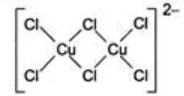
\includegraphics[width=0.3\textwidth]{figure//Cu结构.png}
	\caption{Cu结构}
	\label{fig:Cu结构}
\end{figure}

\ce{CuCl2}不仅易溶于水,而且易溶于有机溶剂,如乙醇,丙酮等。在很高浓度\ce{CuCl2}溶液中,可形成黄色配合物\ce{[CuCl4]^{2-}},显黄色。

$$ \ce{Cu^{2+} + 4Cl- -> [CuCl4]^{2-}} $$

在\ce{CuCl2}稀溶液中,由于被\ce{[Cu(H2O)4]^{2+}}取代,显浅蓝色。

$$ \ce{[CuCl4]^{2-} + 4H2O -> [Cu(H2O)4]^{2+} + 4Cl-} $$

所以,\ce{CuCl2}高浓度溶液常显黄色或黄绿色,这是两种配离子都存在的缘故。

(3)硫酸铜

无水硫酸铜为白色粉末,在水中结晶时为五水合硫酸铜,呈蓝色。五水合硫酸铜(\ce{[Cu(H2O)5]SO4})俗称胆巩,其结构为\ce{[Cu(H2O)4]SO4\cdot H2O},4个水分子与\ce{Cu^{2+}}配位,1个水分子通过氢键与\ce{SO4^{2-}}结合。温度升高,水逐渐脱去。

无水硫酸铜易溶于水,吸水性强,吸水则显出特征性蓝色,可用于测量气体微量水分和作为干燥剂。\ce{CuSO4}由于铜离子水解而呈弱酸性。

\ce{CuSO4}具有杀菌性,可制备波尔多液。\\

3.配合物

(1)\ce{Cu}(I)的配合物:

\ce{Cu}(I)通常形成配位数为2的配合物,常见的有:

\ce{[Cu(SCN)2]+},\ce{[CuCl2]-},\ce{[Cu(NH3)2]+},\ce{[Cu(S2O3)]^{2-}},\ce{[Cu(CN)2]-}

由于\ce{Cu+}的价电子结构为$d^{10}$型,形成的配离子基本无色,大多配合物溶液有吸收\ce{CO}、烯烃、炔烃和释放的能力。

$$ \ce{[Cu(NH2CH2CH2OH)2]+ + C2H4 <=> [Cu(NH2CH2CH2OH)2(C2H4)]+} \Delta _{f}H^{\Theta}_{m}<0$$

该反应常用于石油中分离烯烃。

(2)\ce{Cu}(II)的配合物:

\ce{Cu}(II)与单齿配体通常形成配位数为4的正方形配合物,例如\ce{[CuCl4]2-},\ce{[Cu(NH3)4]^{2+}},\ce{[Cu(H2O)4]^{2+}}。

过量氨水与\ce{Cu^{2+}}盐溶液反应可以生成\ce{[Cu(NH3)4]^{2+}}。

$$ \ce{[Cu(H2O)4]^{2+} + 4NH3 -> [Cu(NH3)4]^{2+} + 4H2O} $$

溶液中\ce{Cu^{2+}}的浓度越小,所形成的蓝色\ce{[Cu(NH3)4)]^{2+}}的颜色越浅,可根据此判断溶液中\ce{Cu^{2+}}含量;\ce{[Cu(NH3)4]^{2+}}有溶解纤维的能力,加入酸或水后纤维又可以析出,工业上利用这种性质制造人造丝。

4.铜(I)与铜(II)的相互转化

虽然\ce{Cu+}为$3d^{10}$结构,但在水溶液中易歧化。由于\ce{Cu^{2+}}所带电荷比\ce{Cu+}多,并且水合焓代数值远远小于\ce{Cu+},所以在水溶液中\ce{Cu+}不如\ce{Cu^{2+}}稳定。

酸性溶液中,\ce{Cu+}的水解常数很大,反应进行得很彻底。而要使\ce{Cu+}转化为\ce{Cu^{2+}},则需要还原剂或者减低\ce{Cu+}的浓度,让它成为难溶物或者难解离的配合物,例如氯化亚铜的制备。

$E_{A}^{\Theta}/V(\ce{Cu^{2+}/CuCl}) 大于 E_{A}^{\Theta}/V(\ce{CuCl/Cu})$,所以\ce{Cu^{2+}}可将\ce{Cu}氧化为\ce{CuCl}。用\ce{SO2}代替\ce{Cu}:

$$ \ce{2Cu^{2+} + SO2 + 2Cl- + 2H2O -> 2CuCl\ce{v} + SO4^{2-} + 4H+} $$

或者\ce{Cu^{2+}}与\ce{KI}反应,可以得到白色的\ce{CuI}沉淀。

$$ \ce{2Cu^{2+} + 4I- -> 2CuI\ce{v} + I2} $$

由于$E^{\Theta}_{A}(\ce{Cu^{2+}/CuI})大于E^{\Theta}_{A}(\ce{I2/I-})$,所以\ce{Cu^{2+}}与\ce{I-}反应得不到沉淀\ce{CuI2},而是得到沉淀\ce{CuI}。

\begin{tcolorbox}
原理:

根据反应电动势与反应常数的关系可知:

$ lgK^{\Theta} = \frac{z\cdot E_{MF}}{0.0592V} $

氧化还原电对电动势越高,反应常数越大,越容易反应完全。所以,生成\ce{CuI}的反应反应常数大于\ce{CuI2}的,生成\ce{CuI}。
\end{tcolorbox}

同样地,向热的\ce{Cu(II)}盐溶液中加入\ce{KCN},可以得到白色的\ce{CuCN}沉淀。

$$ \ce{2Cu^{2+} + 4CN- -> 2CuCN\ce{v} + (CN)2\ce{^}} $$

继续加入过量的KCN,\ce{CuCN}形成\ce{Cu(I)}最稳定的配离子\ce{[Cu(CN)x]^{1-x}}而溶解。

$$ \ce{CuCN + (x-1)CN- -> [Cu(CN)_{x}]^{1-x}} (x=2\sim 4)$$

$\Delta$ 总之,在水溶液中,凡能使\ce{Cu+}生成难溶盐或者稳定\ce{Cu(I)}配离子时,则可使\ce{Cu(II)}转化为\ce{Cu(I)}化合物。


\subsubsection{银的重要化合物}

1.氧化物与氢氧化物

\ce{AgOH}只有用强碱与可溶性银盐的90\%酒精溶液在低于零下40$^\circ C$才能制得。AgOH为白色固体,极不稳定,形成后立即脱水为暗棕色\ce{Ag2O}

$$ \ce{2Ag+ + 2OH- -> Ag2O + H2O} $$

与\ce{Cu2O}相比,\ce{Ag2O}的碱性略强,但是热稳定性差,稍加热便分解为单质和氧。

\ce{Ag2O}既能与硝酸反应,也能溶于氨水,形成二氨合银。

$$ \ce{Ag2O + 4NH3 + H2O -> 2[Ag(NH3)2]+ + 2OH-} $$

2.卤化银

卤化银中只有\ce{AgF}溶于水。卤化银颜色随着\ce{Cl-Br-I}顺序加深,溶解度依次降低。卤化银有感光性,在光照下被分解为单质,先变为紫色,后变为黑色。

$$ \ce{2AgX ->[\text{日光}] 2Ag + X2} $$

\begin{tcolorbox}
原理:

生成的银单质结构松散,没有形成金属晶体,不存在导带,故没有金属光泽,显黑色。

溶解度则是因为阴离子变形性不断增大,极化作用不断增强,共价成分增大,在水中逐渐难溶。

\end{tcolorbox}

\ce{AgBr}可被硫代硫酸钠溶解,形成可溶配合物:

$$ \ce{AgBr + 2S2O3^{2-} -> [Ag(S2O3)2]^{3-} + Br-} $$

该反应曾被用作得到底片。

3.硝酸银

制备:使用蒸发结晶法。

\ce{AgNO3}受热或遇光照容易分解为\ce{NO2}和\ce{O2}。

$$ \ce{2AgNO3 ->[\text{713K或光照}] 2Ag + 2NO2\ce{^} + O2\ce{^}} $$

\ce{AgNO3}具有氧化性,遇微量有机物即被还原为黑色的单质银。

4.配合物

常见与\ce{Ag+}形成二配合物的有:\ce{NH3},\ce{SCN-},\ce{S2O3^{2-}},\ce{CN-},他们形成的配离子稳定性逐渐增加。

\begin{tcolorbox}

原理:

一般来说,单齿配合物稳定性比多齿配合物要强;配体电负性越大,配合键共价性越强,越具有稳定性;配体的分子量越大,与中心原子距离越远,配合键越不稳定。\\

\ce{CN-}是单齿配体,电负性很强,所以稳定性最强;\ce{S2O3^{2-}}虽然为双齿配体,但是电负性较强,其次;\ce{SCN-}虽是单齿配体,但是配位原子可能是\ce{S}也可能是\ce{N},不稳定;\ce{NH3}为单齿,但\ce{N}原子电负性最低,且空间占据大,配合键键长较大,不稳定。

\end{tcolorbox}

二氨合银离子具有弱氧化性,银镜反应:

$$ \ce{2[Ag(NH3)2]+ + RCHO + 3OH- -> 2Ag\ce{v} + RCOO- + 4NH3\ce{^} + 2H2O} $$

\ce{2[Ag(NH3)2]+}放置过程中会变成有爆炸性的\ce{Ag2NH}和\ce{AgN3}。

\subsection{锌族元素}

\subsubsection{锌族元素概述}

1.锌族元素通性

周期表$ds$区包括锌(\ce{Zn})、镉(\ce{Cd})、汞(\ce{Hg})及鎶(\ce{Cn})。\\

对于闪锌矿(\ce{ZnS}),通常使用先焙烧为\ce{ZnO},再用焦炭还原提纯\ce{Zn}。

或者使用湿法,使用硫酸和氧气把\ce{ZnS}转化为\ce{ZnSO4}和硫单质,之后对\ce{ZnSO4}使用电解。\\

锌族元素的价层电子构型均为$(n-1)d^{10}ns^{2}$,由于(n-1)d层电子未成键,所以锌族元素性质与典型过渡元素有较大差别,与p区元素较接近。氧化数主要为+2,汞有+1(总是以双聚离子\ce{[--Hg--Hg--]^{2-}}形式存在),离子无色,金属键较弱,所以硬度低,熔点低。\\

就活泼性而言,除\ce{Hg}之外,\ce{Zn}、\ce{Cd}是较活泼金属;\ce{Zn}和\ce{Cd}的化学性质比较接近,\ce{Hg}与它们相差较大,更接近于铜族元素。\\

锌族元素的\ce{M^{2+}}均无色,所以它们的许多化合物也无色。但是,由于\ce{M^{2+}}具有18电子构型,其极化能力和变形性依\ce{Zn^{2+}--Cd^{2+}--Hg^{2+}}的顺序增强,导致\ce{Cd^{2+}}特别是\ce{Hg^{2+}}与易变形的阴离子形成的化合物,往往显色并具有较低的溶解度。(注:由于锌族元素的阳离子较大较特殊,在判断离子极化时主要考虑其变形性)\\

锌族元素一般都形成较稳定的配合物。

2.锌族单质

锌、镉、汞均为银白色金属,其中锌略带蓝白色。本族元素单质熔沸点较低,并按照从上到下的顺序降低。(原因:同族元素从上到下原子半径增大,金属键减弱)

锌可与其他金属形成许多合金。

汞能溶解许多金属形成汞齐,汞齐是汞的合金。钠汞齐与水反应放出氢,在有机合成中常常用作还原剂。利用汞与金属形成汞齐的特点可从矿石中提取金银等。

锌和镉的化学性质相似,而汞的化学活泼性差很多:

$$ \ce{2Zn + O2 ->[1000^\circ C] 2ZnO} $$
$$ \ce{2Hg + O2 <=>[\text{加热至沸}][500^\circ C] 2HgO} $$

锌在潮湿空气中表面生成一层的致密碱式碳酸盐\ce{Zn(OH)2\cdot ZnCO3}起保护作用,使锌具有防腐蚀的性能。

$$ \ce{2Zn + O2 + H2O + CO2 -> Zn(OH)2\cdot ZnCO3} $$

锌与铝相似,具有两性:

$$ \ce{Zn + 2H+ -> Zn^{2+} + H2\ce{^}} $$
$$ \ce{Zn + 2OH- + 2H2O -> [Zn(OH)4]^{2-} + H2\ce{^}} $$

与铝不同的是,\ce{Zn}能与氨水形成配离子而溶解:

$$ \ce{Zn + 4NH3 + 2H2O -> [Zn(NH3)4](OH)2 + H2\ce{^}} $$

\subsubsection{锌的重要化合物}

1.氧化锌和氢氧化锌

氧化锌(\ce{ZnO})又称锌白,对热稳定,微溶于水,显两性。

在锌盐溶液中,加入适量的碱可析出\ce{Zn(OH)2}沉淀。\ce{Zn(OH)2}也显两性,溶于碱生成锌酸盐:

$$ \ce{Zn(OH)2 + 2OH- -> [Zn(OH)4]^{2-}} $$

也可以溶于氨水,形成配合物:

$$ \ce{Zn(OH)2 + 4NH3 -> [Zn(NH3)4]^{2+} + 2OH-} $$

\begin{tcolorbox}

为什么\ce{Zn}和\ce{Al}拥有两性?\\

与一般的硫酸盐、硝酸盐的组成有很大的不同。对于一般的金属,它们一般表现出金属性,即与由非金属元素与氧组成的酸根阴离子结合;然而像\ce{Zn}、\ce{Al}这样的金属,它们随着原子半径的增大和原子层数的增加,也能表现出一些非金属性,与\ce{O}结合成为阴离子,即常说的两性。

所以,锌酸根可以写作\ce{[Zn(OH)4]^{2-}},也可以写作\ce{ZnO2^{2-}}。

\end{tcolorbox}

2.氯化锌

无水氯化锌为白色固体,可由锌与氯气反应制得。

\ce{ZnCl2}吸水性很强,极易溶于水,水溶液由于锌离子的水解显酸性。

$$ \ce{Zn^{2+} + H2O <=> Zn(OH)+ + H+} $$

在\ce{ZnCl2}的浓溶液中,由于形成配合酸\ce{H[ZnCl2(OH)]},而让溶液具有显著的酸性,甚至能溶解金属氧化物:

$$ \ce{ZnCl2 + H2O -> H[ZnCl2(OH)]} $$

$$ \ce{Fe2O3 + 6H[ZnCl2(OH)] -> Fe[ZnCl2(OH)]3 + 3H2O} $$

在焊接金属前,常用\ce{ZnCl2}的浓溶液清除金属表面的氧化物。\\

要得到无水氯化锌,可用含水氯化锌与氯化亚砜(\ce{SOCl2})一起加热:

$$ \ce{ZnCl2\cdot xH2O + xSOCl2 -> ZnCl2 + 2xHCl + xSO2} $$

3.硫化锌

往锌盐溶液中通入\ce{H2S}时,会生成\ce{ZnS}。

\ce{ZnS}是常见难溶硫化物中唯一呈白色的,与\ce{BaSO4}共同沉淀所形成的混合物晶体\ce{ZnS\cdot BaSO4}叫做锌钡白(俗称立德粉)。\\

在\ce{ZnS}中加入微量\ce{Cu}、\ce{Mg}、\ce{Ag}作活化剂,经光照射后可发出不同颜色的荧光。

4.配合物

\ce{Zn^{2+}}与氨水、氰化钾等可形成无色的四配位的配离子。\\

\ce{[Zn(CN)4]^{2-}}用于电镀工艺。值得注意的是,铜、锌配合物有关电对的标准电极电势相近,所以它们的混合液在电镀时,\ce{Zn}、\ce{Cu}在阴极同时析出,即镀黄铜。

$\Delta$\ce{Zn^{2+}}与二苯硫腙形成稳定的粉色螯合物沉淀,用于鉴定。

\subsubsection{汞的重要化合物}

汞能形成氧化物为+1,+2的化合物,在锌族M(I)的化合物中,以\ce{Hg(I)}的化合物最重要。\\

1.氧化汞

氧化汞有两种红、黄两种变体,都难溶于水,有毒,在500$^\circ C$时分解为汞和氧气。在汞盐溶液中加入碱,可得到黄色\ce{HgO},原因与\ce{Ag}类似,生成的\ce{Hg(OH)2}极不稳定,立即脱水分解。红色的\ce{HgO}则一般由硝酸汞受热分解制得。

$$ \ce{Hg^{2+} + 2OH- -> HgO\ce{v} + H2O} $$

$$ \ce{2Hg(NO3)2 ->[\Delta] 2HgO + 4NO2 + O2\ce{^}} $$

\ce{HgO}是制备许多汞盐的原料。\\

2.氯化汞和氯化亚汞

氯化汞可由在过量氯气中加热汞制得。

\ce{HgCl2}为共价化合物,熔点较低,易生化,俗称升汞。略溶于水,在水中解离度很小,主要以分子形式存在,有“假盐”之称。

\ce{HgCl2}在水中稍微水解:

$$ \ce{HgCl2 + H2O <=> Hg(OH)Cl + HCl} $$

与稀氨水反应则生成难溶的氨基氯化汞:

$$ \ce{HgCl2 + 2NH3 -> Hg(NH2)Cl\ce{v}(\text{白色}) + NH4Cl} $$

\ce{HgCl2}还可以与碱金属氯化物反应形成四氯合汞(II)配离子,让\ce{HgCl2}的溶解度增大。

$$ \ce{HgCl2 + 2Cl- -> [HgCl4]^{2-}} $$

\ce{HgCl2}在酸性溶液中有氧化性,适量的\ce{SnCl2}可以将之还原为难溶于水的白色氯化亚汞。

$$ \ce{2HgCl2 + SnCl2 -> Hg2Cl2\ce{v}(\text{白色}) + SnCl4} $$

分析化学中用此反应鉴定Hg(II)和Sn(II)。\ce{HgCl2}的稀溶液有杀菌作用。\\

金属汞与\ce{HgCl2}固体一起研磨,制得氯化亚汞。

$$ \ce{2Hg + 2HgCl2 -> 2Hg2Cl2} $$

氯化亚汞(\ce{Hg2Cl2}为白色固体,难溶于水。少量的\ce{Hg2Cl2}无毒,俗称甘汞,见光易分解。

$$ \ce{Hg2Cl2 ->[\text{光}] HgCl2 + Hg} $$

\ce{Hg2Cl2}与氨水反应可生成氨基氯化汞和汞,令沉淀显灰色:

$$ \ce{Hg2Cl2 + 2NH3 -> Hg(NH3)Cl\ce{v}(\text{白色}) + Hg(\text{黑色}) + NH4Cl} $$

此反应可用于鉴定\ce{Hg(I)}。\\

3.硝酸汞和硝酸亚汞

硝酸汞\ce{[Hg(NO3)2]}和硝酸亚汞\ce{[Hg2(NO3)2]}都溶于水,并且水解生成碱式盐沉淀。

$$ \ce{Hg(NO3)2 + H2O -> HgO\cdot Hg(NO3)2\ce{v} + 2HNO3} $$

$$ \ce{Hg2(NO3)2 + H2O -> Hg2(OH)NO3\ce{v} + HNO3} $$

所以在配置它们的溶液时,应先溶于稀硝酸中。

在\ce{Hg(NO3)2}中加入\ce{KI}可产生橘红色\ce{HgI2}沉淀,后者溶于过量\ce{KI}中,形成无色\ce{[HgI4]^{2-}}:

$$ \ce{Hg^{2+} + 2I- -> HgI2\ce{v}(\text{橘红色})} $$

$$ \ce{HgI2 + 2I- -> \ce{[HgI4]^{2-}}} $$

同样地,在\ce{Hg2(NO3)2}溶液中加入\ce{KI},先生成浅绿色的\ce{Hg2I2}沉淀,再加入\ce{KI}后形成\ce{[HgI4]^{2-}},同时有汞析出:

$$ \ce{Hg2^{2+} + 2I- -> Hg2I2\ce{v}(\text{浅绿色})} $$

$$ \ce{Hg2I2 +  2I- -> [HgI4]^{2-} + Hg\ce{v}} $$

在\ce{Hg(NO3)2}溶液中加入氨水,可得白色的氨基硝酸汞沉淀。

$$ \ce{2Hg(NO3)2 + 4NH3 + H2O -> HgO\cdot NH2HgNO3\ce{v}(\text{白色}) + 3NH4NO3} $$

在硝酸亚汞中加入氨水会产生上述沉淀和单质汞。

$$ \ce{2Hg2(NO3)2 + 4NH3 + H2O -> HgO\cdot NH2HgNO3\ce{v}(\text{白色}) + 3NH4NO3 + 2Hg(\text{黑色})} $$

\ce{Hg2(NO3)2}受热易分解:

$$ \ce{Hg2(NO3)2 ->[\Delta] 2HgO + 2NO2\ce{^}} $$

由于氧-水电势高于汞离子-亚汞离子的,所以当\ce{Hg2(NO3)2}溶液与空气接触时易被氧化为\ce{Hg(NO3)2}:

$$ \ce{2Hg2(NO3)2 + O2 + 4HNO3 -> 4Hg(NO3)2 + 2H2O} $$

因此可加入少数金属汞避免\ce{Hg2(NO3)2}溶液被氧化。

汞能形成许多稳定的有机化合物,如甲基汞等,它们较易挥发,在空气、水中很稳定。\\

4.配合物

\ce{Hg(I)}形成配合物的倾向较小,\ce{Hg(II)}则易与\ce{Cl-}、\ce{Br-}、\ce{I-}、\ce{CN-}、\ce{SCN-}形成较稳定的配离子,配位数为4。\\

碱性溶液中奈斯勒试剂\ce{K2[HgI4]}是鉴定\ce{NH4+}的特效试剂。根据其与\ce{OH-}相对量的不同,生成褐色(2:4)、深褐色(2:3)、红棕色(2:2)的沉淀。\\

5.\ce{Hg(I)}与\ce{Hg(II)}的转化

汞呈现左大于右电极电势,ce{Hg(I)}不像\ce{Cu(I)}一样容易发生歧化,并且在溶液中\ce{Hg^{2+}}可氧化\ce{Hg}生成\ce{Hg2^{2+}}:

$$ \ce{Hg^{2+} + Hg <=> Hg2^{2+}} \quad K^{\Theta} \approx 88$$

所以平衡时,\ce{Hg^{2+}}基本都转化为\ce{Hg2^{2+}},因此\ce{Hg(II)}化合物用金属汞还原即可得到\ce{Hg(I)}化合物(例如\ce{HgCl2}和\ce{Hg(NO3)2})。

除了用金属汞本身外,还可采用$E^{\Theta}$在一定范围内的还原剂将\ce{Hg(II)}还原为\ce{Hg(I)}。若采用更强的还原剂则需要\ce{Hg(II)}过量。\\

由于归中反应平衡常数较大,为使\ce{Hg2^{2+}}的歧化反应能够进行,必须降低\ce{Hg^{2+}}的浓度,转换为难溶物或稳定配合物,如:

$$ \ce{+ OH- -> HgO\ce{v}} $$

$$ \ce{+ S^{2-} -> HgS\ce{v}} $$

$$ \ce{+ NH3 -> Hg(NH2)Cl\ce{v}} $$

$$ \ce{+ I- -> [HgI4]^{2-}} $$

这些反应在之前均有提及。

除了\ce{Hg2F2}以外,\ce{Hg2X2}都是难溶的(包括拟卤素)。\ce{X-}过量时,才能歧化为\ce{[HgX4]^{2-}}和\ce{Hg}。

\subsection{镧系和锕系}

\subsubsection{镧系和锕系元素概述}

f区元素包含镧系和锕系(57$\sim$ 71、89$\sim$ 102)共28种元素,镧系中只有一个元素是人工合成的,具有放射性;锕系元素则均有放射性。\\

超铀元素:锕系中铀后元素,均为人工合成。\\

稀土元素(RE,Rare Earth):IIIB族中的钇、镥和镧系元素性质非常相似,称为稀土元素,稀土元素分为轻稀土、中稀土、重稀土。\\

f区元素价电子结构:$ (n-2)f^{0\sim 14} (n-1)d^{0\sim 2} ns^2 $,特点是在于随着核电荷数增加,电子填入$ (n-2)f $ 轨道,因此统称内过渡元素。\\

内过渡元素:f区元素。\\

\subsubsection{价层电子构型与氧化数}

镧系元素除\ce{La,Ce,Gd}以外,其他均为$ 4f^x6s^2 $。

镧系元素除了内层4f轨道电子数不同(但能级相近)其他均同,因此性质相似。

形成化合物:镧系元素s、d层电子均可成键,部分4f电子也可成键。镧系元素的第一、二、三电离能总和是比较低的,主要表现出IIIB族元素特征的氧化数(一般形成+3价的化合物,当然也有例外,例如Ba主要形成+2价化合物)。

\subsubsection{原子半径、离子半径和镧系收缩}

镧系收缩、锕系收缩:镧系、锕系元素的原子、离子半径总的趋势是随着原子序数的增加而逐渐减少。\\

1.原子半径:镧系中,电子逐个填充4s亚层,由于4f电子分散,对原子核的屏蔽效应较小,所以随着原子序数的增加,有效核电荷数缓慢增加,原子半径缓慢减小。然而\ce{Eu}和\ce{Yb}的原子半径比较大,这是因为它们的4f电子层分别为半充满和全充满,使得屏蔽作用较强。\\

双峰效应:由于原子半径在\ce{Eu}和\ce{Yb}处的骤升,镧系元素熔点随着原子序数升高,在它们处出现陡降的谷值,而一二三电离能之和则随着原子序数升高出现骤升的升值。\\

\begin{figure}[htpb]
	\centering
	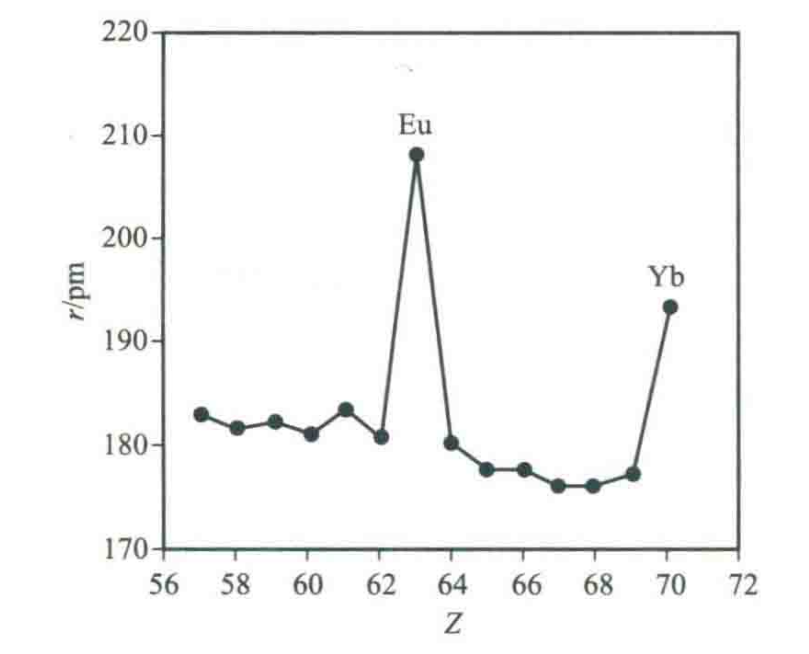
\includegraphics[width=0.5\textwidth]{figure//双峰效应1.png}
	\caption{原子半径的骤升}
	\label{fig:}
\end{figure}

\begin{figure}[htpb]
	\centering
	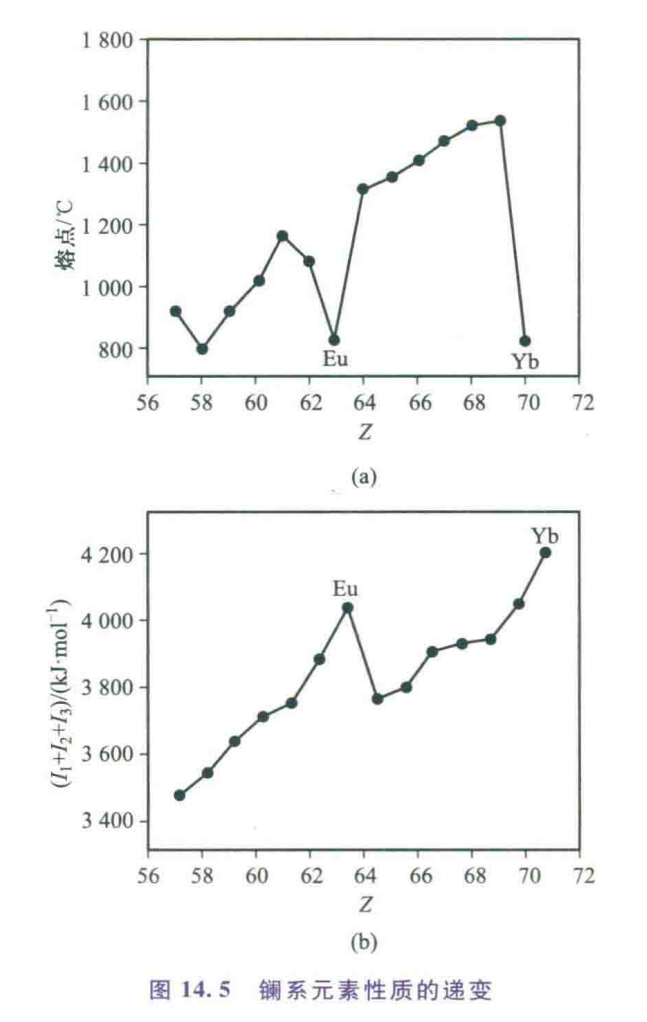
\includegraphics[width=0.5\textwidth]{figure//双峰效应2.png}
	\caption{熔点和一二三电离能总和的“双峰”}
	\label{fig:}
\end{figure}

2.离子半径

与原子半径变化不同,\ce{Ln^3+}的离子半径变化十分有规律,这也导致它们性质极为相似,造成分离上的困难。\\

钇组元素:由于镧系收缩,\ce{Eu}以后的元素性质接近\ce{Y},它们在自然界中共生。\\

\subsubsection{金属活泼性}

镧系元素单质都十分活泼,活泼性与镁相近,且活泼性随着原子序数的增大稍有下降。

与空气反应:金属在空气中被缓慢氧化,加热则容易燃烧,生成\ce{Ln2O3},\ce{Ce}则生成\ce{CeO2}。

与水反应:镧系金属均可与水反应,尤其是热水,反应放出氢气。

与非金属反应:镧系金属可以与大部分非金属反应,反应一般不很剧烈。与卤素加热燃烧生成\ce{LnX3},与氢气加热生成\ce{LnH2}或\ce{LnH3},它们一般属于金属型氢化物。

锕系元素很活泼,它们与沸水作用同时生成氧化物和氢氧化物。它们均可被氢氟酸侵蚀,但大多数仅缓慢与硝酸反应,不与碱发生反应。

\subsubsection{离子的颜色}

按照晶体场理论,f轨道也会发生分裂,当其处于部分填充时,也会发生f-f跃迁,\ce{Ln^3+}的颜色主要由f-f跃迁引起,所以,离子的颜色主要与未成对的f电子数有关。

\subsubsection{离子的磁性}

仅有\ce{La^3+}和\ce{Lu^3+}的未成对电子数为0反磁性,其余均为顺磁性。

\subsection{镧系元素的重要化合物}

\subsubsection{Ln(III)的化合物}

镧系元素化合物体积大,且4f电子被遮蔽,大部分镧系化合物是离子型的。

1.氧化物和氢氧化物

可形成\ce{Ln2O3},颜色与对应离子颜色一致,离子型化合物,熔点很高,均具有碱性,难溶于水,易溶于酸,能形成碱式碳酸盐。

2.盐类

镧系卤化物中仅有\ce{LnF3}不溶于水。

若要制得无水\ce{LnCl3}则需在\ce{HCl}气流中或者过量\ce{NH4Cl}存在下加热。

3.配合物

除了水合离子之外,\ce{Ln^3+}形成配合物的能力不是很强,因为4f被5s,5p轨道屏蔽,离子形成稀有气体结构。又由于半径大,所以配位数一般在6或6以上。

\ce{Ln^3+}与冠醚形成稳定配合物。

\subsection{稀土元素}

稀土元素化学性质活泼,可以溶于碱金属氯化物,与水作用放出氢气。

\subsubsection{稀土元素的应用}

1.冶金工业上,可用于脱氧脱硫,克服氢脆,增加强度,总之牛逼就完事了。

2.汽车和石油化工上,用作废气催化剂或裂化催化剂。

3.做特种玻璃。

4.荧光体和激光材料。

5.制陶业,增强性能,牛逼。

6.电子工业上,用作永磁体。

7.农业上用作化肥,金坷垃牛逼炸了。

\end{document}
